\section{Theorie}
\label{sec:Theorie}

Ein Lock-In-Verstärker (siehe Abbildung \ref{fig:Schaltung1}) dient hauptsächlich der Messung von verrauschten Spannungssignalen.
Das mit der Referenzfrequenz $\omega_0$ modulierte Messsignal $U_{\text{sig}}$ wird im ertsen Schritt durch einen Bandpassfilter geleitet.
Dieser sorgt dafür, dass die rauschenden Oberwellen des Messsignals  mit Frequenzen $\omega >> \omega_0$ und $\omega << \omega$ herausgefiltert werden.
Anschließend wird das Messsignal in einem Mischer mit einer Referenzspannung $U_{\text{ref}}$ multipliziert, deren Amplitude auf 1 nomiert ist.
Die Phasenverschiebung zwischen den beiden Signalen kann über einen Phasenschieber geändert werden und so in Einklang gebracht werden ($\increment\phi = 0$).
Der Mischer sorgt für eine Gleichrichtung des Produkts aus Mess- und Referenzsignal, das bedeutet, dass das Mischsignal nur aus den geraden Oberwellen der Grundfrequenz $\omega_0$ besteht.
Zum Schluss wird das Signal über mehrere Perioden der Modulationsfrequenz $\omega_0$ mit Hilfe eines Tiefpassfilters integriert (Faltung).
Die nicht zur Modulationsfrequenz $\omega_0$ synchronisierten Rauschbeiträge werden sich dadurch größtenteils gegenseitig rausheben.
Am Ausgang wird so eine Gleichspannung gemessen, die proportional zur Eingangsspannung $U_{\text{sig}}$ ist ($U_{\text{out}} \propto U_{\text{sig}} \cos(\phi)$).

Der Tiefpass sollte so gewählt werden, dass die Oberwellen des Signals unterdrückt werden und die Zeitkonstante $\tau = RC >> 1 / \omega_0$ ist.
Durch diese Spezifikation wird die Bandbreite des Rauschanteils $\increment \nu = 1 / (\pi RC)$ sehr klein.
Ein Log-In-Verstärker kann so Güten von $Q = 100.000$ erreichen, im Vergleich zu einem Bandpass der nur Güten von $Q = 1.000$ erreicht.

Wird für die Referenzspannung $U_{\text{ref}}$ ein Sinussignal gewählt und für die Eingangsspannung $U_{\text{sig}}$ auch, in der Form
\begin{equation}
  U_{\text{sig}} = U_0 \sin(\omega t),
  \label{eqn:gl1}
\end{equation}
ergibt sich für die Ausgangsspannung $U_{\text{out}}$ folgende Proportionalität zur Spannung des Messsignals:
\begin{align}
  U_{\text{out}} = \frac{2}{\pi} U_0
  \label{eqn:gl2}
  \intertext{bzw. für eine feste Phasenverschiebung:}
  U_{\text{out}} = \frac{2}{\pi} U_0 \cos(\phi)
  \label{eqn:gl3}
\end{align} \cite{V303}

\begin{figure}
  \centering
  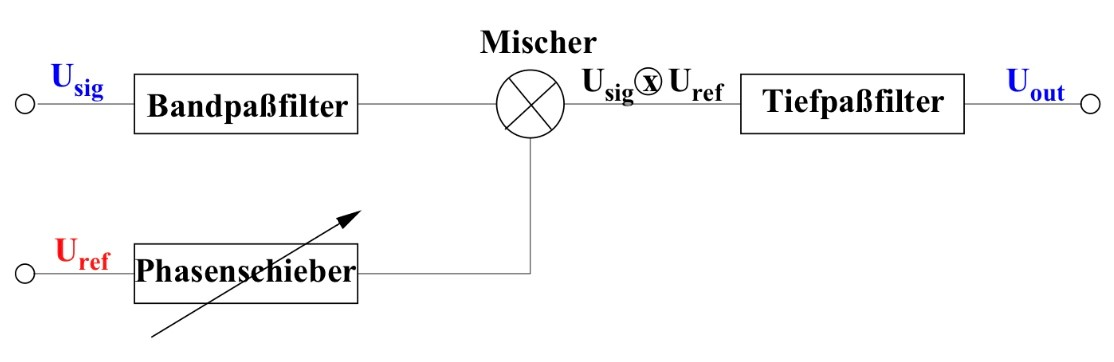
\includegraphics[width=\textwidth]{data/Schaltung1.jpg}
  \caption{Schematischer Aufbau eines Lock-In-Verstärkers \cite{V303}}
  \label{fig:Schaltung1}
\end{figure}
